\documentclass{article}
\usepackage[fleqn]{amsmath}
\usepackage{latexsym}
\usepackage{amsfonts}
\usepackage{amssymb}
\usepackage{graphicx}


\begin{document}


\section{Simulation Studies}
\subsection{Experimental Setup}
We evaluate the performance of our algorithm via simulation in this section.
Our simulation setting is as follows. We randomly create $n$(ranged from $50$ to $150$) nodes
on a $100*100\,m^2$ square ~\cite{Maxi}. The data sinks are also randomly located within this square. The maximum rate for each sensor is $100\,Kbps$. The maximum transmission range of each sensor is $25\,m$. For power consumption model, we set $e_{Rx} = 0.00002\,J/b$, $e_{Tx} = 0.00003\,nJ/b$ ~\cite{Wire}. Since nodes in our protocol do not 
consume more energy than they can collect, the rate nodes are directly related to the amount of energy that they collect. Take solar energy as an example ~\cite{Ste} . The total energy collected from a $37 * 33\,mm^2$ solar cell over a 48-h period is $655.15\,mWh$ for the sunny day and $313.70\,mWh$ for the partly cloudy day. Thus we generate $B_V(t+1)$ for every sensor node randomly between $8.19\,J$ and $3.92\,J$ with every $10\,mins$ for a timeslot. We also set each sensor with a $2AA$ Battery for initial.\\
We compare the performance and running time of our algorithm(\textbf{TPath}) with the Garg and K\"{o}nemann's framework algorithm(\textbf{Garg and K\"{o}nemann}). We run each experiment over 20 different topologies.

\subsection{Impact of $\epsilon$ on Performance}

\begin{figure}[H]
\centering
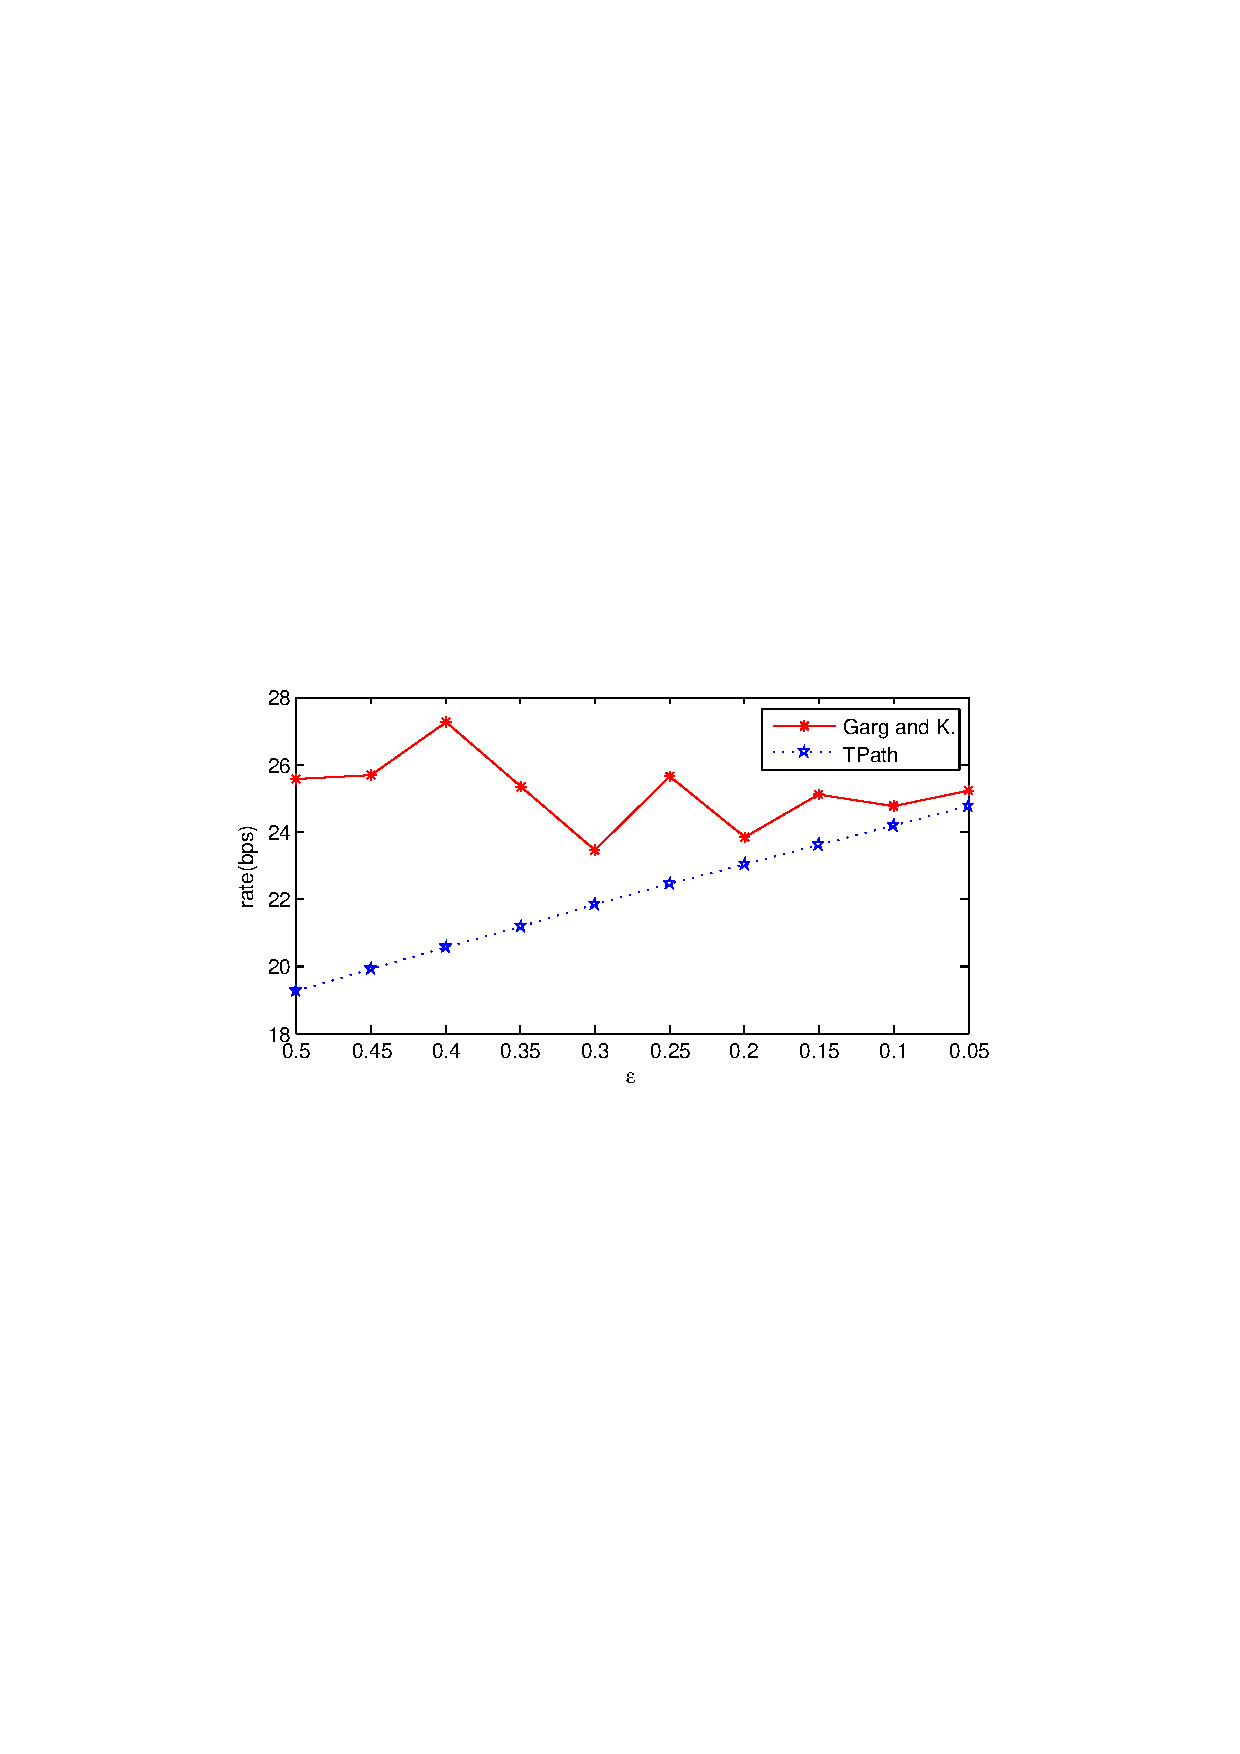
\includegraphics[scale=0.6]{performance.pdf} 
\caption{Impact of $\epsilon$}
\label{f1}
\end{figure}

First we show the impact of $\epsilon$, the parameter of the approximation algorithm, on the network performance. We run both algorithms of different $\epsilon$ over 20 different random topologies. Each topology is randomly generated including $100$ sensor nodes on a $100*100\,m^2$ square. From figure~\ref{f1}, we observe that with the $\epsilon$ fall from 0.5 to 0.05, the performance between two algorithms are smaller. The interesting result shows that our algorithm could performance as well as the Garg and K\"{o}nemann's framework algorithm with proper approximation parameter.

\subsection{Running Time}

\begin{figure}[H]
\centering
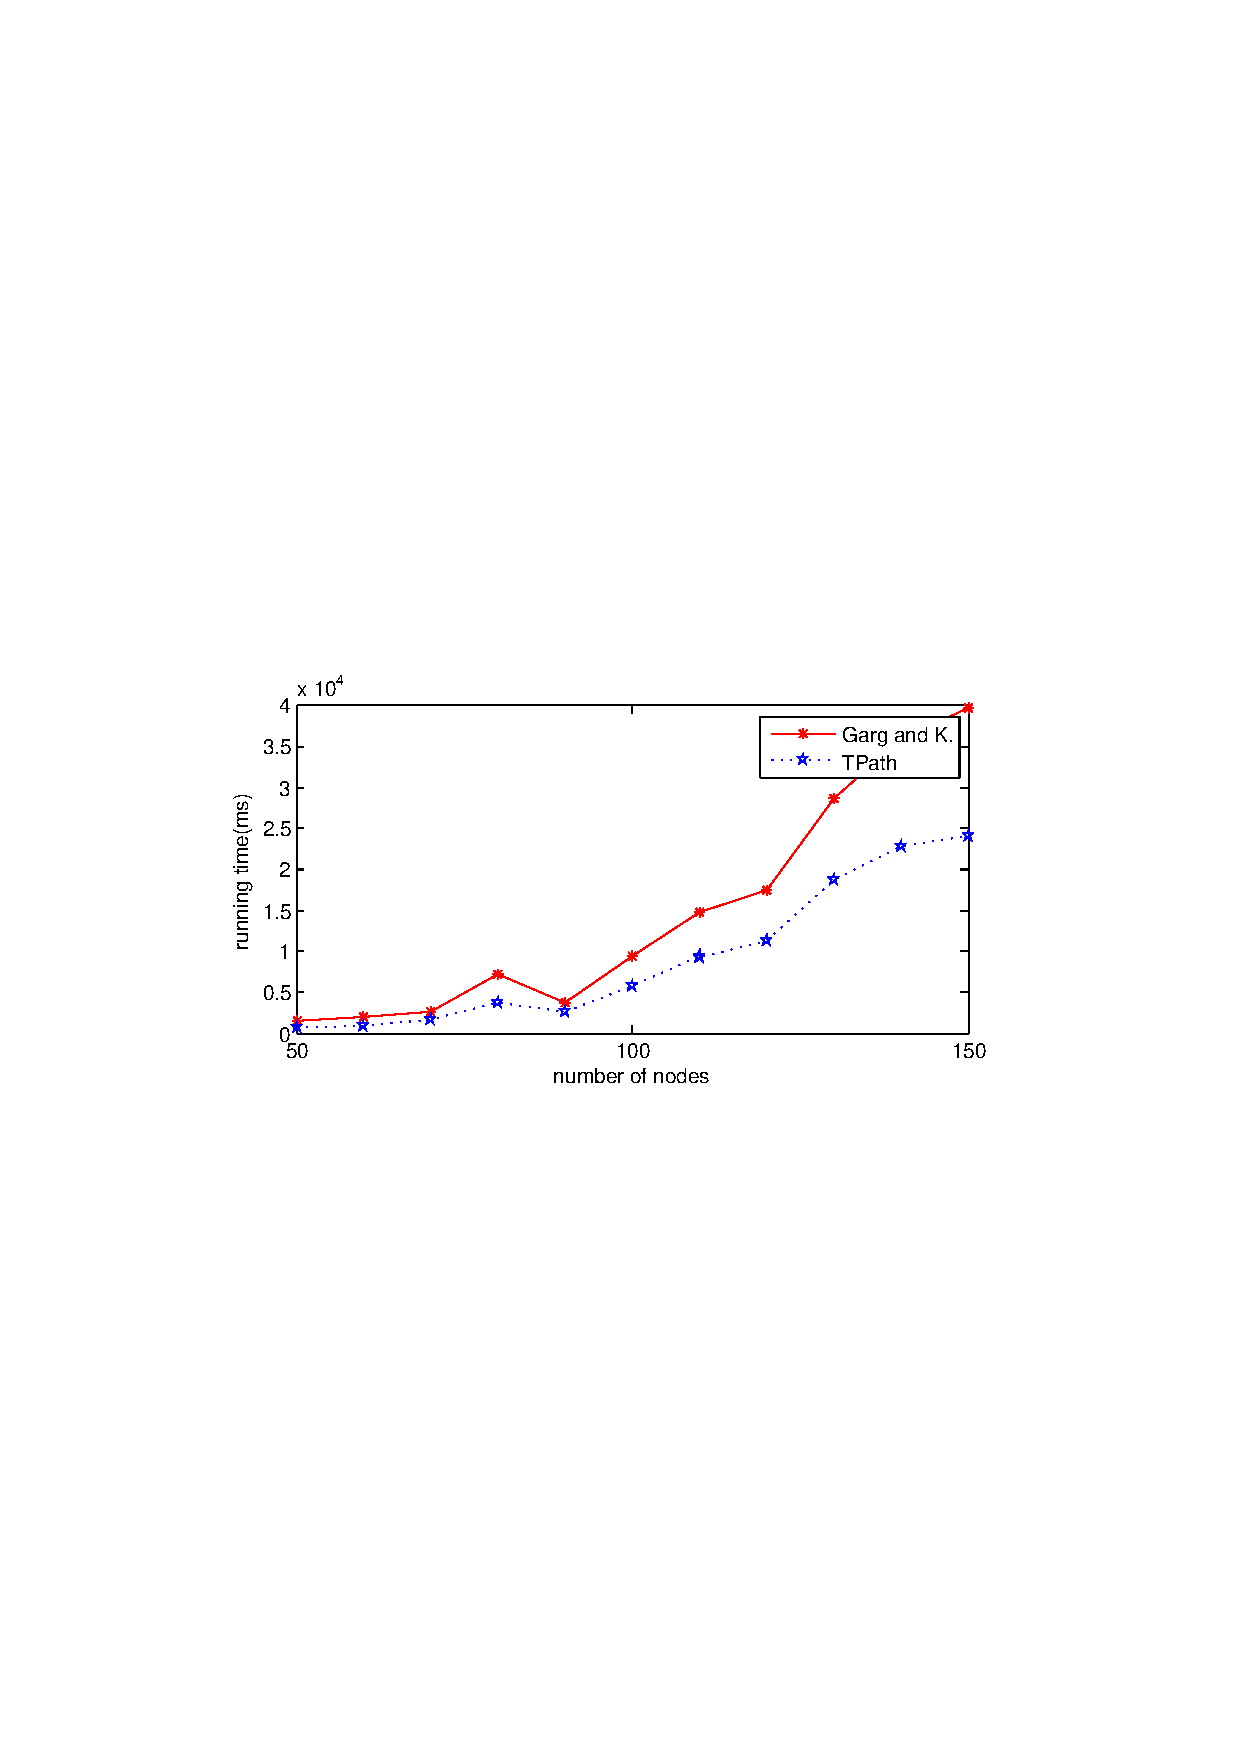
\includegraphics[scale=0.6]{running.pdf} 
\caption{Comparison of running time}
\label{f2}
\end{figure}
From above section, it shows that our algorithm could performance as well as the Garg and K\"{o}nemann's framework algorithm with proper $\epsilon$(e.g. $\epsilon = 0.1$). Then we evaluate the running time of both algorithms by $\epsilon =0.1$ in a test-bed with a processor running at $2.40\,GHz$ and $3.86\,GB$ RAM over 20 different topologies of which the nodes number ranged from 50 to 150.
Figure~\ref{f2} shows that the running time growth of both algorithms when the sensor nodes increaseing from 50 to 150. Obviously, running time is a key feature especially in large-scale network. The result shows that the Garg and K\"{o}nemann's framework algorithm 
grows much faster than our algorithm. Our explanation for such a phenomenon is as follows. The Garg and K\"{o}nemann's framework algorithm compute shortest path per node per loop, while our algorithm only do shortest path computing one time per loop through the $DS(e)$ assistance. 


\bibliographystyle{plain}
\bibliography{Maxi,Ste,Wire}


\end{document}